\section{热传递 传导}\label{sec:2-5}

生活经验告诉我们,插在热汤里的金属勺,它的把很快会烫手;
放在炉火上的一壶冷水,不久会被烧开;
坐在篝火旁边的人们,身体会被烤暖。
可见,热可以从温度高的物体传到温度低的物体,或者从物体的高温部分传到低温部分。
这种现象叫做\textbf{热传递}。

实验表明,\CJKunderwave{只要物体之间或同一物体的不同部分存在着温度差,
就会有热传递现象发生,并且将一直继续到温度相同的时候为止}。
由于种种原因,物体之间或同一物体的不同部分,温度常常是不同的。
所以,热传递是一种普遍存在的自然现象。

人们经过长期研究知道,\CJKunderwave{热传递的方式有三种:传导,对流,辐射}。
我们先研究传导。

照图 \ref{fig:2-13} 那样,用凡士林在金属棒上粘几根火柴,然后用酒精灯给金属棒的 $A$ 端加热。
可以看到,离 $A$ 端最近的火柴先掉下,然后其他几根火柴依次掉下,离 $A$ 端越远的火柴掉下得越迟。
这表明,热是从金属棒的温度高的一端沿着金属棒传到温度低的一端去的。

\begin{figure}[htbp]
    \centering
    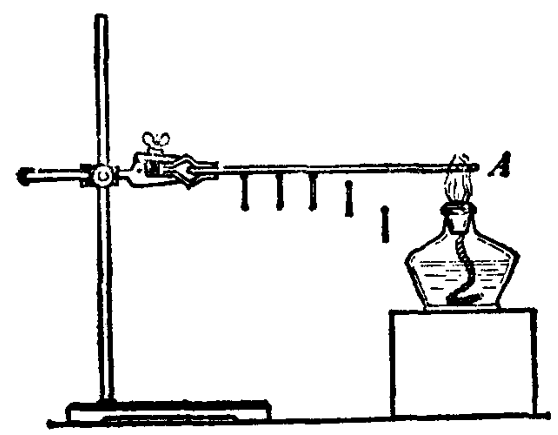
\includegraphics[width=0.5\textwidth]{../pic/czwl2-ch2-13}
    \caption{传导}\label{fig:2-13}
\end{figure}

热从物体的温度较高的部分沿着物体传到温度较低的部分,叫做\textbf{传导}。

各种物质都能够传热,但是不同物质的传热本领不同。

把金属勺放在热汤里面,勺把很快就烫手,可是把瓷勺、木筷子、竹筷子放在热汤里面,
它们很久也不烫手。这表明金属善于传热,瓷、木头和竹子不善于传热。

拿一个装着凉水的试管,照图 \ref{fig:2-14} 那样给试管上部的水加热。
上面的水已经开了,下面的水还不烫手。这表明水不善于传热。

\begin{figure}[htbp]
    \centering
    \begin{minipage}{7cm}
    \centering
    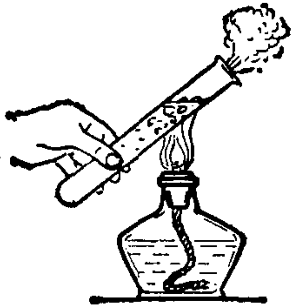
\includegraphics[width=4cm]{../pic/czwl2-ch2-14}
    \caption{水不善于传热}\label{fig:2-14}
    \end{minipage}
    \qquad
    \begin{minipage}{7cm}
    \centering
    \vspace{1cm}
    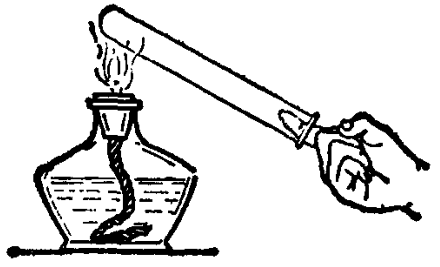
\includegraphics[width=5cm]{../pic/czwl2-ch2-15}
    \caption{空气不善于传热}\label{fig:2-15}
    \end{minipage}
\end{figure}


照图 \ref{fig:2-15} 那样让试管口斜向下方,给试管底部的空气加热,把手指放在试管口处,
过了相当久,手指还不觉得热。这表明空气不善于传热。

我们把善于传热的物质叫做热的良导体。
各种金属都是热的良导体,其中最善于传热的是银,其次是铜和铝。
不善于传热的物质叫做热的不良导体,
瓷、纸、木头、玻璃、皮革都是热的不良导体。
最不善于传热的是羊毛、羽毛、毛皮、棉花、石棉、软木和其他松软的物质。
液体,除了水银以外,都不善于传热,气体比液体更不善于传热。
冬天穿棉衣、皮衣觉得暖和,就是因为在棉花、毛皮的纤维中间有不流动的空气,身体的热不容易散失掉。

